% Options for packages loaded elsewhere
% Options for packages loaded elsewhere
\PassOptionsToPackage{unicode}{hyperref}
\PassOptionsToPackage{hyphens}{url}
\PassOptionsToPackage{dvipsnames,svgnames,x11names}{xcolor}
%
\documentclass[
  english,
  10pt,
  letterpaper,
  DIV=11,
  numbers=noendperiod]{scrartcl}
\usepackage{xcolor}
\usepackage[margin=1in]{geometry}
\usepackage{amsmath,amssymb}
\setcounter{secnumdepth}{5}
\usepackage{iftex}
\ifPDFTeX
  \usepackage[T1]{fontenc}
  \usepackage[utf8]{inputenc}
  \usepackage{textcomp} % provide euro and other symbols
\else % if luatex or xetex
  \usepackage{unicode-math} % this also loads fontspec
  \defaultfontfeatures{Scale=MatchLowercase}
  \defaultfontfeatures[\rmfamily]{Ligatures=TeX,Scale=1}
\fi
\usepackage{lmodern}
\ifPDFTeX\else
  % xetex/luatex font selection
\fi
% Use upquote if available, for straight quotes in verbatim environments
\IfFileExists{upquote.sty}{\usepackage{upquote}}{}
\IfFileExists{microtype.sty}{% use microtype if available
  \usepackage[]{microtype}
  \UseMicrotypeSet[protrusion]{basicmath} % disable protrusion for tt fonts
}{}
\makeatletter
\@ifundefined{KOMAClassName}{% if non-KOMA class
  \IfFileExists{parskip.sty}{%
    \usepackage{parskip}
  }{% else
    \setlength{\parindent}{0pt}
    \setlength{\parskip}{6pt plus 2pt minus 1pt}}
}{% if KOMA class
  \KOMAoptions{parskip=half}}
\makeatother
% Make \paragraph and \subparagraph free-standing
\makeatletter
\ifx\paragraph\undefined\else
  \let\oldparagraph\paragraph
  \renewcommand{\paragraph}{
    \@ifstar
      \xxxParagraphStar
      \xxxParagraphNoStar
  }
  \newcommand{\xxxParagraphStar}[1]{\oldparagraph*{#1}\mbox{}}
  \newcommand{\xxxParagraphNoStar}[1]{\oldparagraph{#1}\mbox{}}
\fi
\ifx\subparagraph\undefined\else
  \let\oldsubparagraph\subparagraph
  \renewcommand{\subparagraph}{
    \@ifstar
      \xxxSubParagraphStar
      \xxxSubParagraphNoStar
  }
  \newcommand{\xxxSubParagraphStar}[1]{\oldsubparagraph*{#1}\mbox{}}
  \newcommand{\xxxSubParagraphNoStar}[1]{\oldsubparagraph{#1}\mbox{}}
\fi
\makeatother


\usepackage{longtable,booktabs,array}
\newcounter{none} % for unnumbered tables
\usepackage{calc} % for calculating minipage widths
% Correct order of tables after \paragraph or \subparagraph
\usepackage{etoolbox}
\makeatletter
\patchcmd\longtable{\par}{\if@noskipsec\mbox{}\fi\par}{}{}
\makeatother
% Allow footnotes in longtable head/foot
\IfFileExists{footnotehyper.sty}{\usepackage{footnotehyper}}{\usepackage{footnote}}
\makesavenoteenv{longtable}
\usepackage{graphicx}
\makeatletter
\newsavebox\pandoc@box
\newcommand*\pandocbounded[1]{% scales image to fit in text height/width
  \sbox\pandoc@box{#1}%
  \Gscale@div\@tempa{\textheight}{\dimexpr\ht\pandoc@box+\dp\pandoc@box\relax}%
  \Gscale@div\@tempb{\linewidth}{\wd\pandoc@box}%
  \ifdim\@tempb\p@<\@tempa\p@\let\@tempa\@tempb\fi% select the smaller of both
  \ifdim\@tempa\p@<\p@\scalebox{\@tempa}{\usebox\pandoc@box}%
  \else\usebox{\pandoc@box}%
  \fi%
}
% Set default figure placement to htbp
\def\fps@figure{htbp}
\makeatother


% definitions for citeproc citations
\NewDocumentCommand\citeproctext{}{}
\NewDocumentCommand\citeproc{mm}{%
  \begingroup\def\citeproctext{#2}\cite{#1}\endgroup}
\makeatletter
 % allow citations to break across lines
 \let\@cite@ofmt\@firstofone
 % avoid brackets around text for \cite:
 \def\@biblabel#1{}
 \def\@cite#1#2{{#1\if@tempswa , #2\fi}}
\makeatother
\newlength{\cslhangindent}
\setlength{\cslhangindent}{1.5em}
\newlength{\csllabelwidth}
\setlength{\csllabelwidth}{3em}
\newenvironment{CSLReferences}[2] % #1 hanging-indent, #2 entry-spacing
 {\begin{list}{}{%
  \setlength{\itemindent}{0pt}
  \setlength{\leftmargin}{0pt}
  \setlength{\parsep}{0pt}
  % turn on hanging indent if param 1 is 1
  \ifodd #1
   \setlength{\leftmargin}{\cslhangindent}
   \setlength{\itemindent}{-1\cslhangindent}
  \fi
  % set entry spacing
  \setlength{\itemsep}{#2\baselineskip}}}
 {\end{list}}
\usepackage{calc}
\newcommand{\CSLBlock}[1]{\hfill\break\parbox[t]{\linewidth}{\strut\ignorespaces#1\strut}}
\newcommand{\CSLLeftMargin}[1]{\parbox[t]{\csllabelwidth}{\strut#1\strut}}
\newcommand{\CSLRightInline}[1]{\parbox[t]{\linewidth - \csllabelwidth}{\strut#1\strut}}
\newcommand{\CSLIndent}[1]{\hspace{\cslhangindent}#1}

\ifLuaTeX
\usepackage[bidi=basic,shorthands=off]{babel}
\else
\usepackage[bidi=default,shorthands=off]{babel}
\fi
\ifLuaTeX
  \usepackage{selnolig} % disable illegal ligatures
\fi


\setlength{\emergencystretch}{3em} % prevent overfull lines

\providecommand{\tightlist}{%
  \setlength{\itemsep}{0pt}\setlength{\parskip}{0pt}}



 


\KOMAoption{captions}{tableheading}
\makeatletter
\@ifpackageloaded{caption}{}{\usepackage{caption}}
\AtBeginDocument{%
\ifdefined\contentsname
  \renewcommand*\contentsname{Table of contents}
\else
  \newcommand\contentsname{Table of contents}
\fi
\ifdefined\listfigurename
  \renewcommand*\listfigurename{List of Figures}
\else
  \newcommand\listfigurename{List of Figures}
\fi
\ifdefined\listtablename
  \renewcommand*\listtablename{List of Tables}
\else
  \newcommand\listtablename{List of Tables}
\fi
\ifdefined\figurename
  \renewcommand*\figurename{Figure}
\else
  \newcommand\figurename{Figure}
\fi
\ifdefined\tablename
  \renewcommand*\tablename{Table}
\else
  \newcommand\tablename{Table}
\fi
}
\@ifpackageloaded{float}{}{\usepackage{float}}
\floatstyle{ruled}
\@ifundefined{c@chapter}{\newfloat{codelisting}{h}{lop}}{\newfloat{codelisting}{h}{lop}[chapter]}
\floatname{codelisting}{Listing}
\newcommand*\listoflistings{\listof{codelisting}{List of Listings}}
\makeatother
\makeatletter
\makeatother
\makeatletter
\@ifpackageloaded{caption}{}{\usepackage{caption}}
\@ifpackageloaded{subcaption}{}{\usepackage{subcaption}}
\makeatother
\usepackage{bookmark}
\IfFileExists{xurl.sty}{\usepackage{xurl}}{} % add URL line breaks if available
\urlstyle{same}
% fallback for those not using the hyperref driver hyperxmp:
\makeatletter
\@ifundefined{xmpquote}{\newcommand{\xmpquote}[1]{#1}}{}
\makeatother
\hypersetup{
  pdftitle={Lévy-Powered Bounded Factors},
  pdfauthor={Complex--Itô Random-Walk Research Project},
  pdflang={en},
  pdfkeywords={\xmpquote{stochastic correlation}, \xmpquote{Levy
processes}, \xmpquote{variance-gamma}, \xmpquote{normal inverse
Gaussian}, \xmpquote{Feynman-Kac integro-differential
equation}, \xmpquote{Gil-Pelaez inversion}},
  colorlinks=true,
  linkcolor={blue},
  filecolor={Maroon},
  citecolor={Blue},
  urlcolor={Blue},
  pdfcreator={LaTeX via pandoc}}


\title{Lévy-Powered Bounded Factors}
\usepackage{etoolbox}
\makeatletter
\providecommand{\subtitle}[1]{% add subtitle to \maketitle
  \apptocmd{\@title}{\par {\large #1 \par}}{}{}
}
\makeatother
\subtitle{What Survives of Exact Correlation Laws under Jump Drivers}
\author{Complex--Itô Random-Walk Research Project}
\date{August 21, 2026}
\begin{document}
\maketitle
\begin{abstract}
We replace the Gaussian driver of a bounded-factor correlation model by
pure-jump Lévy processes (variance-gamma, normal-inverse-Gaussian) and
determine layer by layer what survives. Marginal laws survive exactly:
\(\rho_T=f(x_0+L_T)\) pushes the closed-form Lévy law through the
Jacobian, and digitals price by Gil--Pelaez inversion ---
deterministically. The clock characteristic function
\(E[e^{i\xi\int_0^T\rho_sds}]\) survives via the \emph{backward}
Feynman--Kac integro-differential equation, valid precisely because
time-homogeneous Lévy drivers retain semigroup time-translation
invariance (the failure mode recently documented for deterministic
coefficient curves does not bite); we solve it with implicit Euler and a
single precomputed LU factorization, handling infinite activity through
the standard small-jump compensation and an effective diffusion.
Reflection-principle barrier laws die honestly: jumps cross levels
without touching. Scientifically, jump asymmetry is a first-order driver
of correlation risk: variance-matched variance-gamma with \(\theta<0\)
roughly halves the mean occupation integral (\(0.073\to0.035\)), and NIG
with \(\beta<0\) flips its sign --- a falsifiable signature invisible to
any marginal-only analysis. All transforms are verified against
closed-form anchors (integrated characteristic exponents; tiny-jump
Gaussian limit), exact samplers validated against their own exponents,
and Monte Carlo within one to two standard errors.
\end{abstract}

\renewcommand*\contentsname{Table of contents}
{
\setcounter{tocdepth}{2}
\tableofcontents
}

\textbf{Mathematics Subject Classification (2020):} 60H10, 60G51, 91G20,
65N30.

\textbf{JEL classification:} G13, C63.

\section{Introduction}\label{sec-introduction}

Jump-driven correlation is empirically plausible --- dependence breaks
in crashes --- yet the audited stochastic-correlation literature
contains no Lévy-driven model: hyperbolic-OU families (Teng et al. 2016)
are Gaussian to the core, and affine jump models price returns or
volatilities, not a bounded dependence coordinate. This paper builds the
missing object and maps, exactly, which laws of the Gaussian theory
transfer.

Driver: \(X_t=x_0+b\,t+L_t\) with \(L\) variance-gamma or NIG; factor
\(\rho_t=X_t/\sqrt{X_t^2+c^2}\).

\section{What survives}\label{sec-survival}

\subsection{Marginal laws: exact}\label{marginal-laws-exact}

\(\rho_T=f(x_0+L_T)\) pushes the closed-form Lévy law through the
monotone Jacobian \(c(1-\rho^2)^{-3/2}\). With \(\psi(u)\) the
log-characteristic exponent,

\[
P(\rho_T\ge\rho^*)=1-\Big[\tfrac12-\tfrac1\pi\int_0^\infty
\operatorname{Im}\big(e^{-iu x^*}e^{T\psi(u)}\big)\frac{du}{u}\Big],
\]

\(x^*=x(\rho^*)-x_0\): exact up to quadrature tolerance. Verified
against exact samplers (VG via gamma subordination with \(E[G_t]=t\);
NIG via inverse-Gaussian subordination) at all quartiles within 0.01.

\subsection{Clock transform: exact via backward
FK-PIDE}\label{clock-transform-exact-via-backward-fk-pide}

For time-\emph{homogeneous} drivers the semigroup is
translation-invariant, so the backward equation is legitimate --- the
failure documented for deterministic coefficient curves is a
time-dependence phenomenon:

\[
\partial_tu=b\,\partial_xu+\int\!\big[u(x+y)-u(x)-y\partial_xu\,
1_{|y|<1}\big]\nu(dy)+q(x)u,\qquad u(0,x)=1 .
\]

We solve on localized grids with implicit Euler and \textbf{one
precomputed LU} (the operator is time-independent). Infinite activity:
exclude a single grid step, folding its mass into a compensating drift
\(b_{\text{eff}}=b-m_1(\epsilon)\) and an effective diffusion
\(\tfrac12\sigma_\epsilon^2\partial_{xx}\),
\(\sigma_\epsilon^2=\int_{|y|<\epsilon}y^2\nu(dy)\) --- for NIG this
term carries most of the process variance at practical grid spacings and
is not optional. Two implementation bugs caught by our own anchors are
recorded in Section~\ref{sec-anchors}.

\subsection{Barrier laws: dead}\label{barrier-laws-dead}

Reflection requires continuous paths; jumps cross levels without
touching. Barrier pricing under jumps needs absorbing-type PIDEs ---
noted as the honest casualty, out of scope here.

\section{Closed-form anchor}\label{sec-anchor}

With linear potential \(f(x)=x\), stochastic Fubini gives

\[
E\Big[e^{iu\int_0^TX_sds}\Big]
=\exp\Big(iu(x_0T+bT^2/2)+T\int_0^1\psi(uT(1-r))\,dr\Big),
\]

an independent correctness target for the PIDE solver (agreement within
0.01 after discretization) --- and, in the tiny-jump limit, recovery of
the Gaussian forward-FK solver of the companion paper (\textless0.02).

\section{Findings}\label{sec-findings}

Variance-matched comparison at \(T=1\), \(c=1\), \(b=0.15\)
((\textbf{tab-clocks?})):

{\def\LTcaptype{none} % do not increment counter
\begin{longtable}[]{@{}
  >{\raggedright\arraybackslash}p{(\linewidth - 6\tabcolsep) * \real{0.2500}}
  >{\raggedright\arraybackslash}p{(\linewidth - 6\tabcolsep) * \real{0.2500}}
  >{\raggedright\arraybackslash}p{(\linewidth - 6\tabcolsep) * \real{0.2500}}
  >{\raggedright\arraybackslash}p{(\linewidth - 6\tabcolsep) * \real{0.2500}}@{}}
\toprule\noalign{}
\begin{minipage}[b]{\linewidth}\raggedright
\(\xi\)
\end{minipage} & \begin{minipage}[b]{\linewidth}\raggedright
Gaussian
\end{minipage} & \begin{minipage}[b]{\linewidth}\raggedright
VG PIDE (MC)
\end{minipage} & \begin{minipage}[b]{\linewidth}\raggedright
NIG PIDE (MC)
\end{minipage} \\
\midrule\noalign{}
\endhead
\bottomrule\noalign{}
\endlastfoot
0.5 & +0.9949+0.0334j & +0.9960+0.0092j (+0.9960+0.0087j) &
+0.9948−0.0243j (+0.9949−0.0220j) \\
1.0 & +0.9796+0.0660j & +0.9841+0.0187j (+0.9840+0.0177j) &
+0.9793−0.0478j (+0.9798−0.0432j) \\
2.0 & +0.9204+0.1255j & +0.9384+0.0388j (+0.9383+0.0369j) &
+0.9196−0.0895j (+0.9214−0.0807j) \\
\end{longtable}
}

\begin{enumerate}
\def\labelenumi{\arabic{enumi}.}
\tightlist
\item
  \textbf{Halved clock mean}: VG with \(\theta=-0.12\) gives
  \(E[A_T]=0.0350\) vs Gaussian \(0.0730\) --- marginal calibration of
  the driver does not pin down path-dependent correlation risk.
\item
  \textbf{Sign flip}: NIG with \(\beta=-2\) makes
  \(\operatorname{Im}\phi_A(\xi)<0\): negative average correlation from
  a driver whose marginals match a positive-correlation Gaussian
  specification (Figure~\ref{fig-clock}).
\end{enumerate}

\begin{figure}[tbp]

\centering{

\pandocbounded{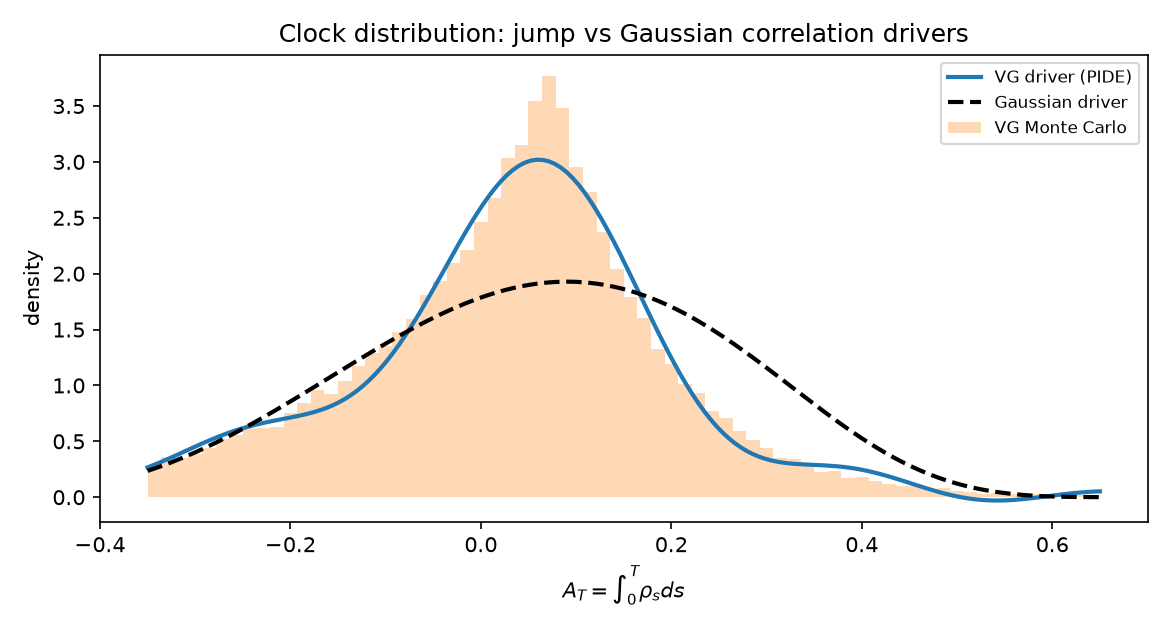
\includegraphics[keepaspectratio]{figures/phase11_clock_densities.png}}

}

\caption{\label{fig-clock}Clock densities under jump vs Gaussian
drivers: Fourier-inverted PIDE transforms vs MC histogram.}

\end{figure}%

\section{Implementation anchors}\label{sec-anchors}

Two silent-corruption bugs were caught by requiring samplers and
exponents to agree: (i) the gamma subordinator's scale parameter must be
\(\nu\) (so \(E[G_t]=t\)), not unity; (ii) exponent functions are
\emph{characteristic} exponents --- real arguments are frequencies, and
passing imaginary arguments silently produced real-valued garbage. We
also record that a gradient-compensation term added on top of shifted
convolution weights double-counts the truncated first moment and biases
the process mean by exactly the Lévy-mean contribution. These are
exactly the failure classes that marginal-only validation misses.

\section{Related literature}\label{sec-related}

Lévy-driven stochastic volatility is standard (Bates; NIG-GARCH); Lévy
drivers of a \emph{bounded dependence coordinate} are absent from the
audited corpus. FK integro-differential theory is classical (Sato 1999);
Gil--Pelaez inversion and small-jump approximations are standard tools;
our contribution is their assembly into an exact pricing stack for
correlation, plus the survival/collapse analysis.

\section{Conclusion}\label{sec-conclusion}

Jumps cost the reflection toolkit but not the transform stack. The
practical message is sharp: calibrating a correlation model's marginals
--- under any driver --- says almost nothing about its path-dependent
risk, and jump asymmetry moves the latter by economically large factors.

\section{Reproducibility}\label{sec-repro}

Environment: conda \texttt{phase3-paper} (Python 3.12.13, numpy 2.5.1,
scipy 1.18.0). Notebook \texttt{notebooks/phase11\_levy.ipynb}
(\textasciitilde321 s, seed 20260821); module \texttt{phase11\_levy.py};
tests \texttt{tests/test\_phase11\_levy.py} (9/9).

\protect\phantomsection\label{refs}
\begin{CSLReferences}{1}{1}
\bibitem[\citeproctext]{ref-sato1999}
Sato, Ken-iti. 1999. \emph{L{é}vy Processes and Infinitely Divisible
Distributions}.

\bibitem[\citeproctext]{ref-teng2016}
Teng, Long, Matthias Ehrhardt, and Michael Günther. 2016. {``Modelling
Stochastic Correlation.''} \emph{Journal of Mathematics in Industry} 6
(1): 1--18. \url{https://doi.org/10.1186/s13362-016-0018-4}.

\end{CSLReferences}




\end{document}
